\documentclass[a4paper]{article}

\usepackage[utf8]{inputenc}
\usepackage{erk}
\usepackage{times}
\usepackage{graphicx}
\usepackage[top=22.5mm, bottom=22.5mm, left=22.5mm, right=22.5mm]{geometry}

\usepackage[slovene,english]{babel}
\usepackage{hyperref}
\usepackage{url}

\let\oldfootnotesize\footnotesize
\renewcommand*{\footnotesize}{\oldfootnotesize\scriptsize}

\begin{document}
\title{seminar 2\\ POROČILO IZDELAVE IGRE - AIRBORNE \\
 Računalniška grafika in tehnologija iger, FRI 2022}

\author{Luka Uranič$^{1} (63200035)$, Alen Kurtagić$^{1} (04200012)$,  Ana Maurič$^{1} (64190013)$, \\ Anja Jerala$^{2}$,  Nika Črne$^{2}$} % use ^1, ^2 for author(s) from different institutions

\affiliation{	$^{1}$Univerza v Ljubljani, Fakulteta za računalništvo in informatiko \\ 
				$^{2}$Univerza v Ljubljani, Naravoslovnotehniška fakuteta}

\maketitle

\selectlanguage{slovene}

\begin{abstract}{Abstract}
Airborne je letalska igra, narejena v Unity-ju. Je izboljšana in nadgrajena igra verzije, narejene v WEB-GLju. S to verzijo igre smo želeli izboljšati grafiko, uvesti bolj kompleksno logiko, povečati natančnost in predvsem izboljšati uporabniško izkušnjo. Delo je bilo razdeljeno podobno kot pri prvem seminarju - to sta dva osnovna dela: oblikovanje in izvoz modelov (rakete, otokov, žetonov, goriva, oblakov) v Blenderju ter programiranje igre v Unityju. Pomagali smo si z veliko tutoriali na internetu (Youtube in ostale spletne strani z Unity tutoriali in nasveti). Celotno delo je trajalo približno 2 tedna. 
\begin{center}
     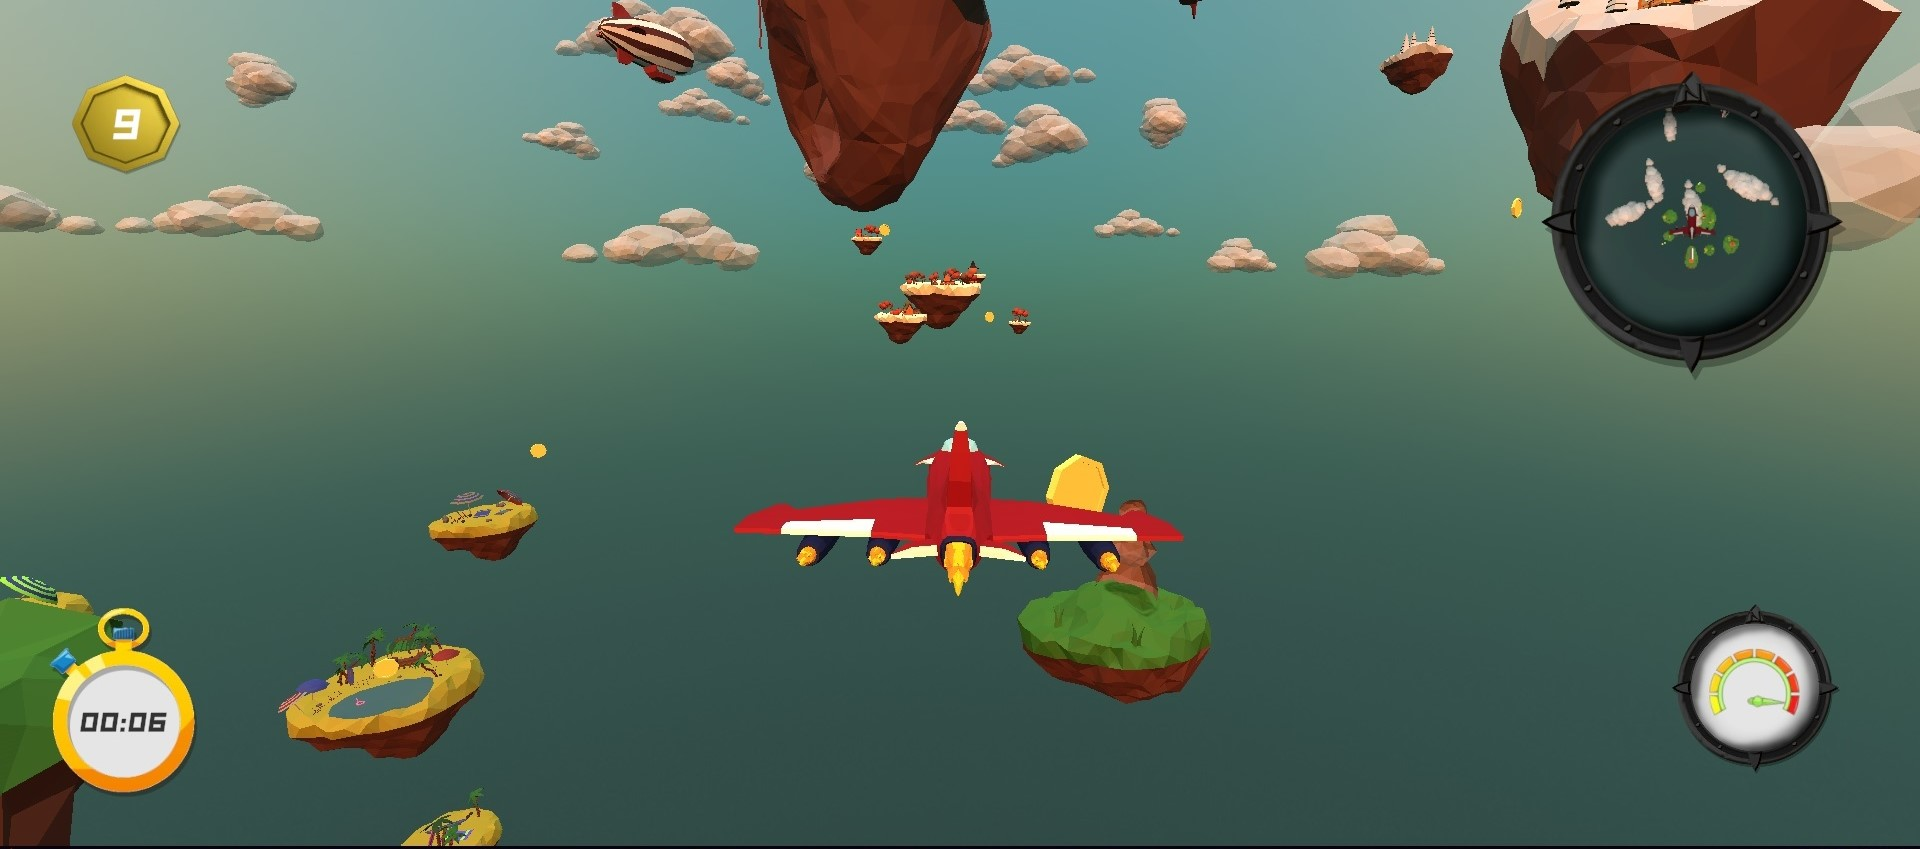
\includegraphics[width=\columnwidth]{game.jpg}
\end{center}
\end{abstract}

\section{Pregled igre}
Igra Airborne je letalska igra iz izbrane perspektive - 1. ali 3. osebe, po želji igralca. V primerjavi s prvim seminarjem smo spremenili cilj igre - igralec usmerja raketo, s katero poskuša nabrati določeno število žetonov v čim krajšem času. Vmes mora pobirati tudi gorivo. Igralec izgubi, ko se  zaleti v ovire v svetu ali pa ko mu zmanjka goriva. Igralec mora biti dovolj spreten, da se približa žetonom ali gorivom in jih pobere, brez da se zaleti v ovire, ki so postavljene blizu obojega. Žetoni tokrat ne predstavljajo goriva, v tem seminarju smo ju ločili med sabo. Raketo lahko usmerja v vse smeri neba, prav tako pa spreminja hitrost same rakete. Tudi ta verzija je namenjena vsem, ki si jo želijo igrati, izkušeni igralci kot tudi začetniki. Raketa začne na lebdeči ploščadi, giblje se po nebu, okrog nje so lebdeči otoki, oblaki, kantice goriva in zlati žetoni, v ozadju je sončno obzorje. Cilj igre oz. zmaga, je pobrati vseh 9 zahtevanih žetonov v najkrajšem možnem času. 

\subsection{Opis sveta}
Naš 3D svet je tokrat upodobljen z bolj dodelanimi 3D modeli z več podrobnostmi - novi otoki so narejeni po navdihu 4 letnih časov, to so poletni, jesenski, zimski in pomladni otoki. Vsak otok ima na sebi nekaj, kar upodablja ta letni čas. Okoli otokov se generirajo zlati žetoni in rdeče kantice goriva. Prav tako smo dodali začetno ploščad oz. Hangar, kjer raketa nabere hitrost in začne svoj let. Igralec nima več letala, ampak raketo (ki se še vedno lahko premika kamorkoli po xyz oseh). Ohranili smo bele prozorne oblake na nebu. V daljavi v neskončnosti se vidi sončno obzorje.

\subsubsection{Pregled}
Glaven model v svetu je raketa. Igralec lahko izbere, ali jo bo videl iz 3. perspetive, ali pa se bo postavil v kabino oz. 1. perspektivo. Igralec se ves čas igre nahaja na sredini zaslona. Z dviganjem, spuščanjem, rotiranjem in obračanjem se približuje in oddaljuje otokom, žetonom, gorivom, oblakom in ozdaju. V zgornjem levem kotu ekrana se nahaja odštevalec pobranih žetonov. V zgrornjem desnem kotu je zemljevid, ki kaže položaj rakete iz ptičje perspektive. V spodnjem levem kotu je štoparica, v spodnjem desnem pa še merilec goriva. Hitrosti ne prikazujemo več.

\subsubsection{Ozadje}
Za ozadje smo uporabili zastonjsko Unity teksturo, naloženo v "Asset Library". Je statična slika, prikazuje barven ombre efekt obzorja.

\subsubsection{Ključne lokacije}
Ključna lokacija v svetu je sredina, kjer se nahaja kar nekaj lebdečih otokov. Samo na tej lokaciji lahko igralec najde žetone in goriva, za letalo predstavlja nahajališče dobrin, ostalo je samo ozadje - kot je podrobneje opisano v drugih razdelkih, sta to ne-interaktivno sončno obzorje in tla. Na tej točki je igra še vedno zelo podobna prejšnjemu seminarju.

\subsubsection{Velikost}
Svet je večji od sveta prejšnjega seminarja - vsebuje 4 vrste otokov, med katerimi je več prostora. Na ta svet gledamo iz 1. ali 3. perspektive, da si ga lahko v celoti ogledamo in obiščemo. 

\subsubsection{Objekti}
Vsi modeli, ki sestavljajo naš svet, so narejeni v Blenderju. Naredili sta jih oblikovalki Nika in Anja. Modele smo vnesli v Unity, jih postavili v pravo mapo ("Models") in enako naredili z njihovimi materiali (v mapo "Materials"). Modeli so podrobneje predstavljeni v razdelku "Osebek", ostali objekti, ki pa zajemajo ozadje, pa v razdelku "Ozadje". 

\subsubsection{Čas}
Hitrost časa v našem svetu ni čisto enaka realnemu času - sekunde sicer minevajo enako, let rakete je pa za potrebe te igre časovno krajši kot let resnične rakete/letala. 

\subsection{Igralni pogon in uporabljene tehnologije}
Uporabljene tehnologije za izdelavo igre so bile Blender in Unity, za deljenje kode pa platforma Github.

\subsection{Pogled}
Kot že predstavljeno, je Airborne igra iz 1. in 3. perspektive. Igralec lahko tako s tipko 2 vidi naš model rakete ali pa se postavi v samo srce akcije s tipko 1. Kamera je vezana oz. pozicionirana glede na raketo, ker je to igralčev objekt premikanja. Vedno bo igralec pred seboj videl okolico in opcijsko tudi raketo. Kot gledanja je širok, da lahko še vedno vidi čim več okolice.

\section{Osebek}
Glavni osebek v igri je raketa. Je rdeče in bele barve z animiranim ogenjčkom. Igralec jo usmerja s tipkami WASD, SPACE in LEFT SHIFT - W/S za dol/gor, A/D za levo/desno. Z tipko SPACE se pospešek poveča, z LEFT SHIFT pa zmanjša. 

\begin{center}
     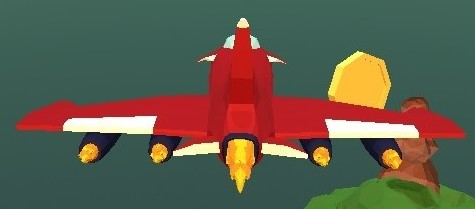
\includegraphics[width=\columnwidth]{raketa.jpg}
\end{center}

Lebdeči otoki se nahajajo se v večjem številu na sredini sveta, okoli rakete. Imamo 4 skupine otokov (za vsak letni čas), vsaki skupini pripada 4 do 6 posameznih otokov. Glavni otok za jesen ima na sebi kočo, drevesa in buče. Za pomlad ima hiško z urejenim dvoriščem. Za poletje bazen z palmami, ležalniki in stojnico. Za zimo pa zasneženo smučišče. Poleg glavnih otokov so tudi manjši, na katerih so skale, drevesa ipd. Igra vsebuje še otok pridelovalnice goriva, in hangar, začetno postajo rakete. Predstavljajo glavno oviro za raketo - če se zaleti vanj ali v njegove predmete, eksplodira in igre je konec. 
\begin{center}
     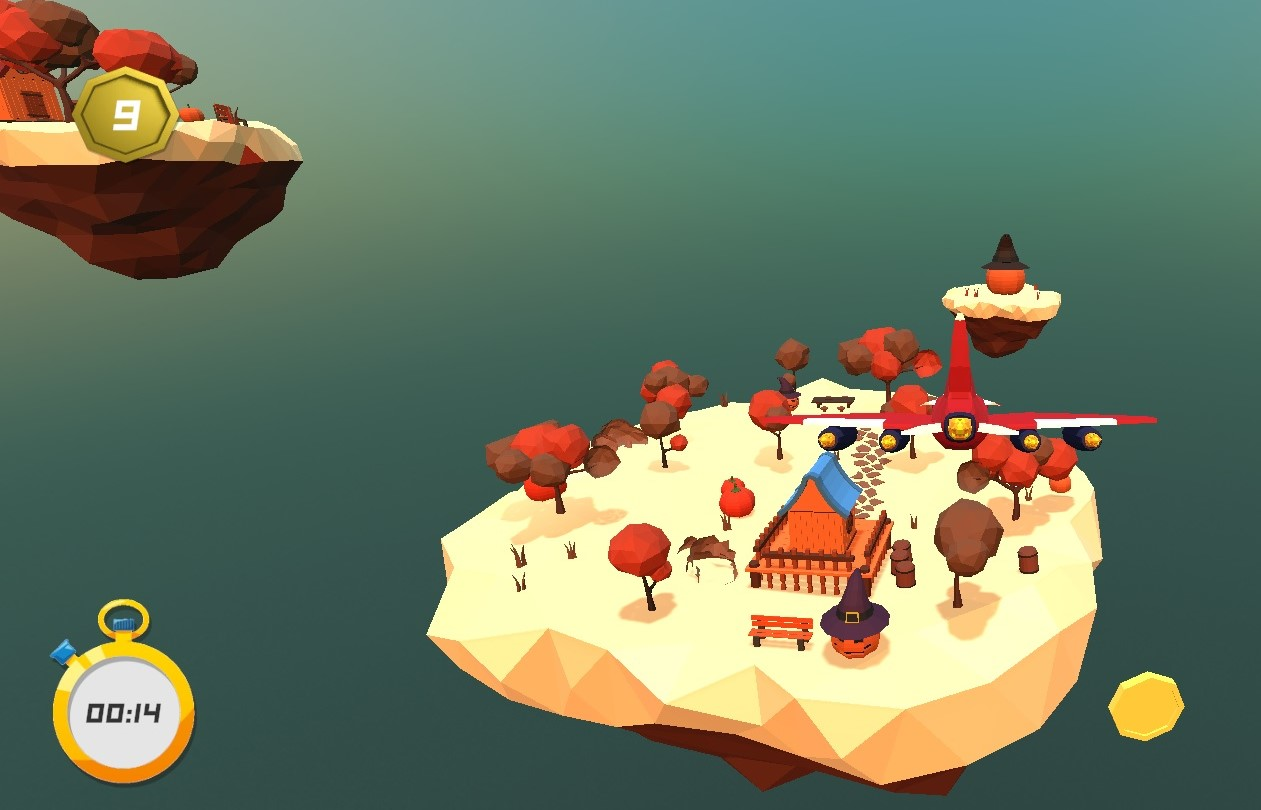
\includegraphics[width=\columnwidth]{autumn.jpg}
\end{center}

Žetoni so glavni objekt za interakcijo z raketo, generirajo se po svetu. Ko jih pobere, se mu za eno številko zmanjša odštevalnik žetonov.
\begin{center}
     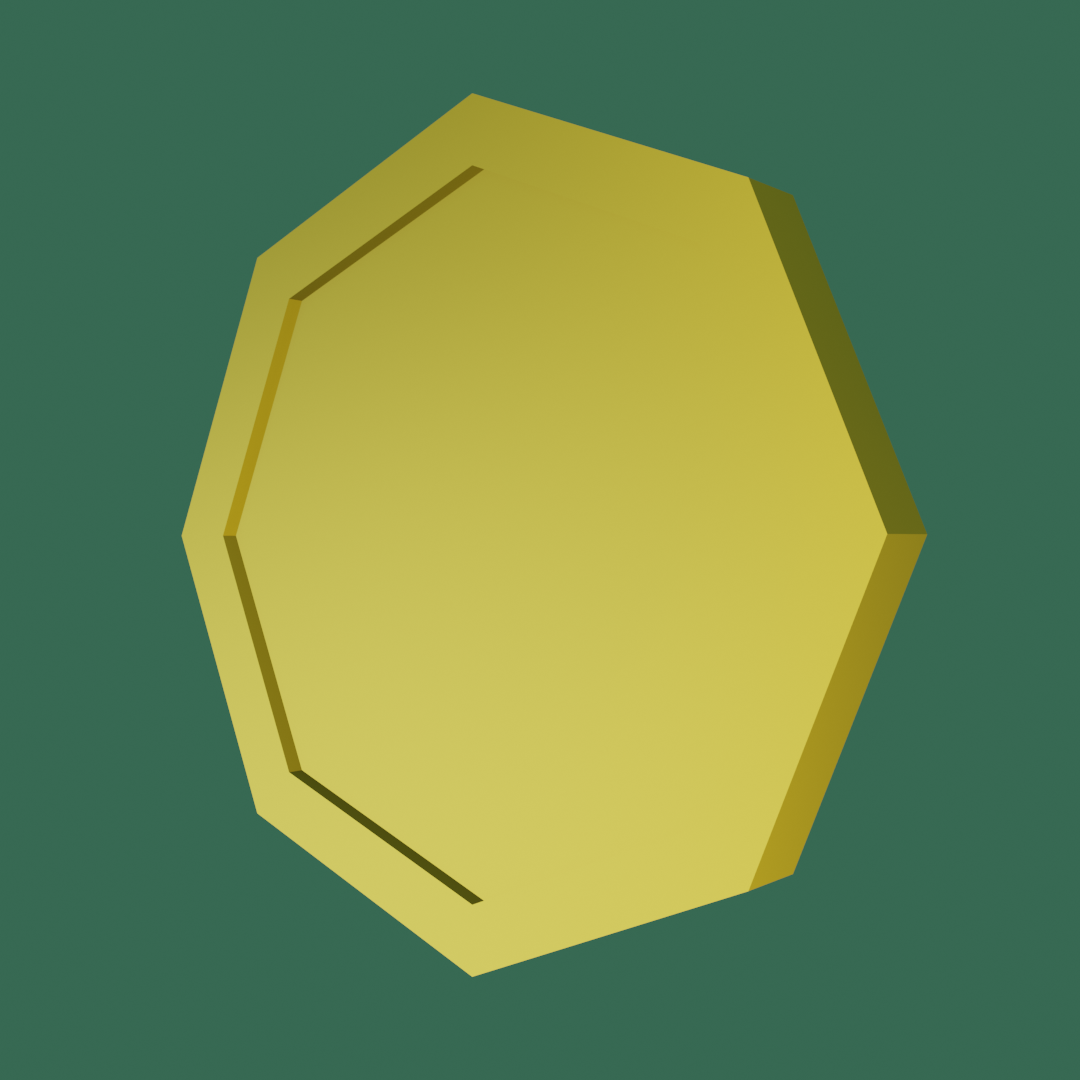
\includegraphics[width=\columnwidth]{coin1.jpg}
\end{center}

Kantice bencina so drugi najpomembnejši objekt za raketo, imajo statično mesto pojavljanja. Spadajo pod naftni otok. Med letom naj bi igralec pobral vsaj eno kantico. Ko jo, se mu poveča meter goriva.
\begin{center}
     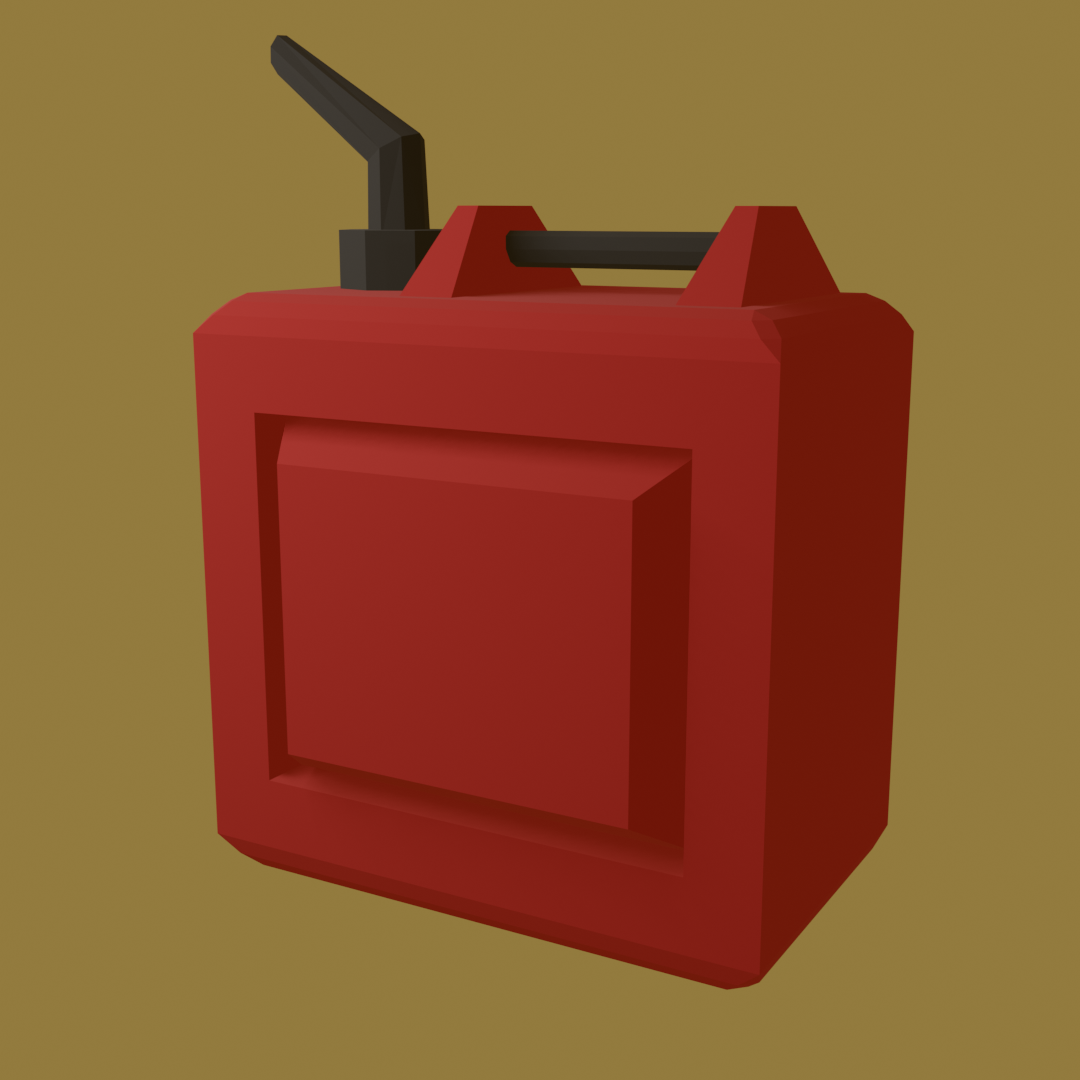
\includegraphics[width=\columnwidth]{bzn.jpg}
\end{center}

Za okras smo dodali tudi animiran leteči Zeppelin (v katerega se prav tako raketa ne sme zaleteti). 
\begin{center}
     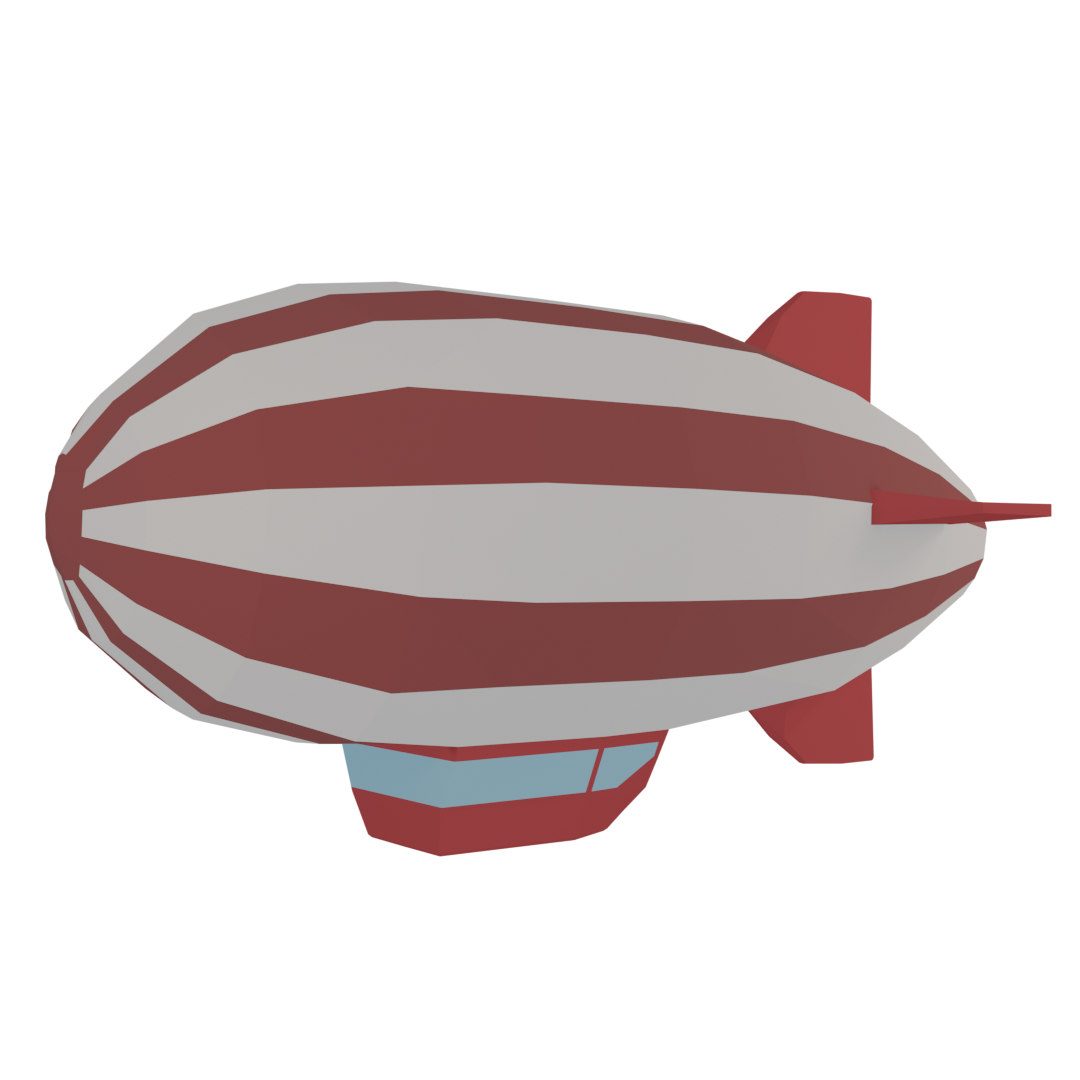
\includegraphics[width=\columnwidth]{zeppelin.jpg}
\end{center}

Preostanejo še oblaki, ki pa obstajajo le za realističen pridih. Niso ovire in hkrati letalu nič ne doprinesejo. Letalo lahko za zabavo leti skozi njih. Generirajo se naključno po določenem intervalu, tudi premikajo se. Ko so izven zaslona, se uničijo.
\begin{center}
     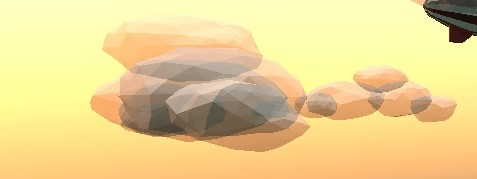
\includegraphics[width=\columnwidth]{oblaki.jpg}
\end{center}

Na otoke, oblake, gorivo, zeppelin in žetone igralec nasploh ne more vplivati zunaj tega, da se jih dotakne. 

\section{Uporabniški vmesnik}
Igralec uporablja miško z ikono rumenega kurzorja in tipke WASD, SPACE in LEFT SHIFT za premikanje rakete. Kot opisano pod razdelkom "Pregled", lahko igralec med igro vidi št. preostalih žetonov, zemljevid, uro in preostalo gorivo.

\section{Glasba in zvok}
Uporabljamo 4 zvočne efekte:
Zvok raketnega motorja igra med letom rakete, glede na pospešek se jakost zvoka skupaj z njim veča ali manjša. Začne se predvajati ko prvič igralec pritisne na tipko SPACE. Vir: \footnote{\url{https://mixkit.co/free-sound-effects/rocket}}
Ko igralec pobere žeton, zaigra vesel žvenketajoč zvok. Vir: \footnote{\url{https://www.youtube.com/watch?v=FJWA77bSlt8&ab_channel=F09F92A6McJulianB.TulibasF09F92A6}}
Ob zmagi se zasliši vesel zvočni efekt. Vir: \footnote{\url{https://www.youtube.com/watch?v=uNwomOkKefM&ab_channel=GFXSounds}}
Zadnji je še zvok eksplozije ob izgubi igre. Vir: \footnote{\url{https://www.youtube.com/watch?v=i76ZNjeoJBU&ab_channel=VideoPlasty}}

\section{Gameplay}
Pred začetkom igre se pred igralcem pojavi hangar z raketo. Zgoraj vidi naslov igre AIRBORNE, v spodnjem levem kotu zlato uro, v spodnjem desnem pa tipko PLAY. Ko pritisne na PLAY, ga odnese v 3. perspektivo za raketo, pritisne lahko SPACE in požene raketo. Nato jo premika s tipkami WASD, kot opisano pod razdelkom "Osebek". Ko pobere 9 žetonov ga spet odnese na začetno stran, kjer lahko v zlati uri vidi svoj čas. Igro lahko ponovno igra kolikokrat želi.

\begin{center}
     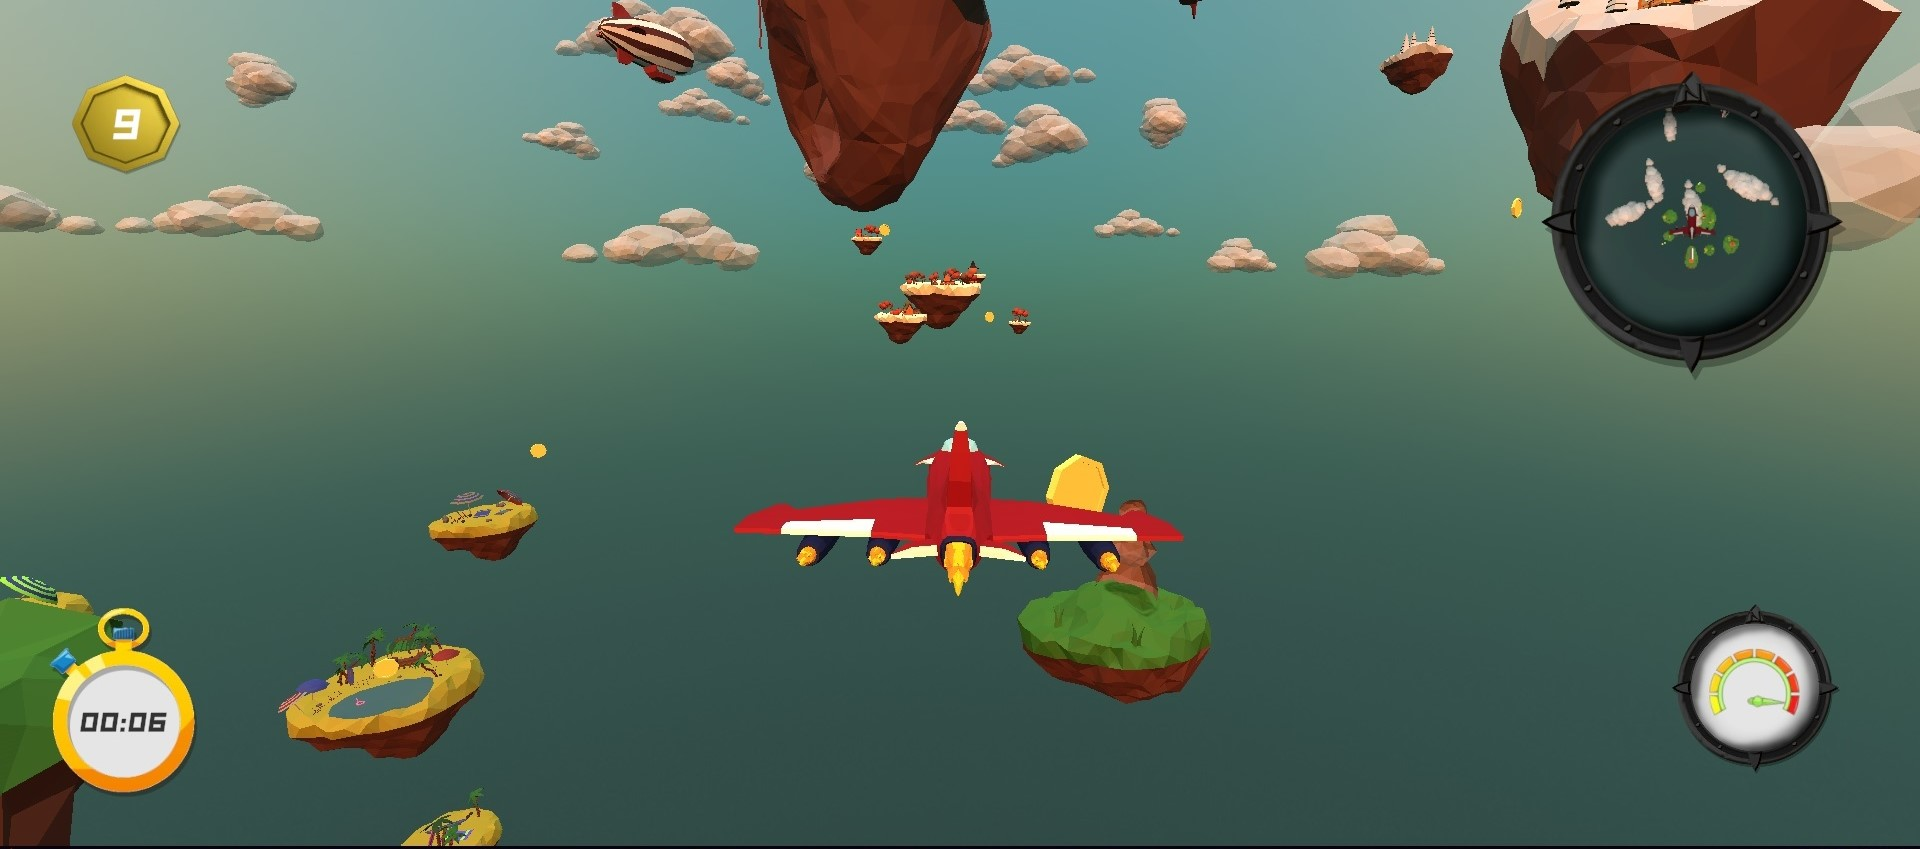
\includegraphics[width=\columnwidth]{game.jpg}
\end{center}

\begin{center}
     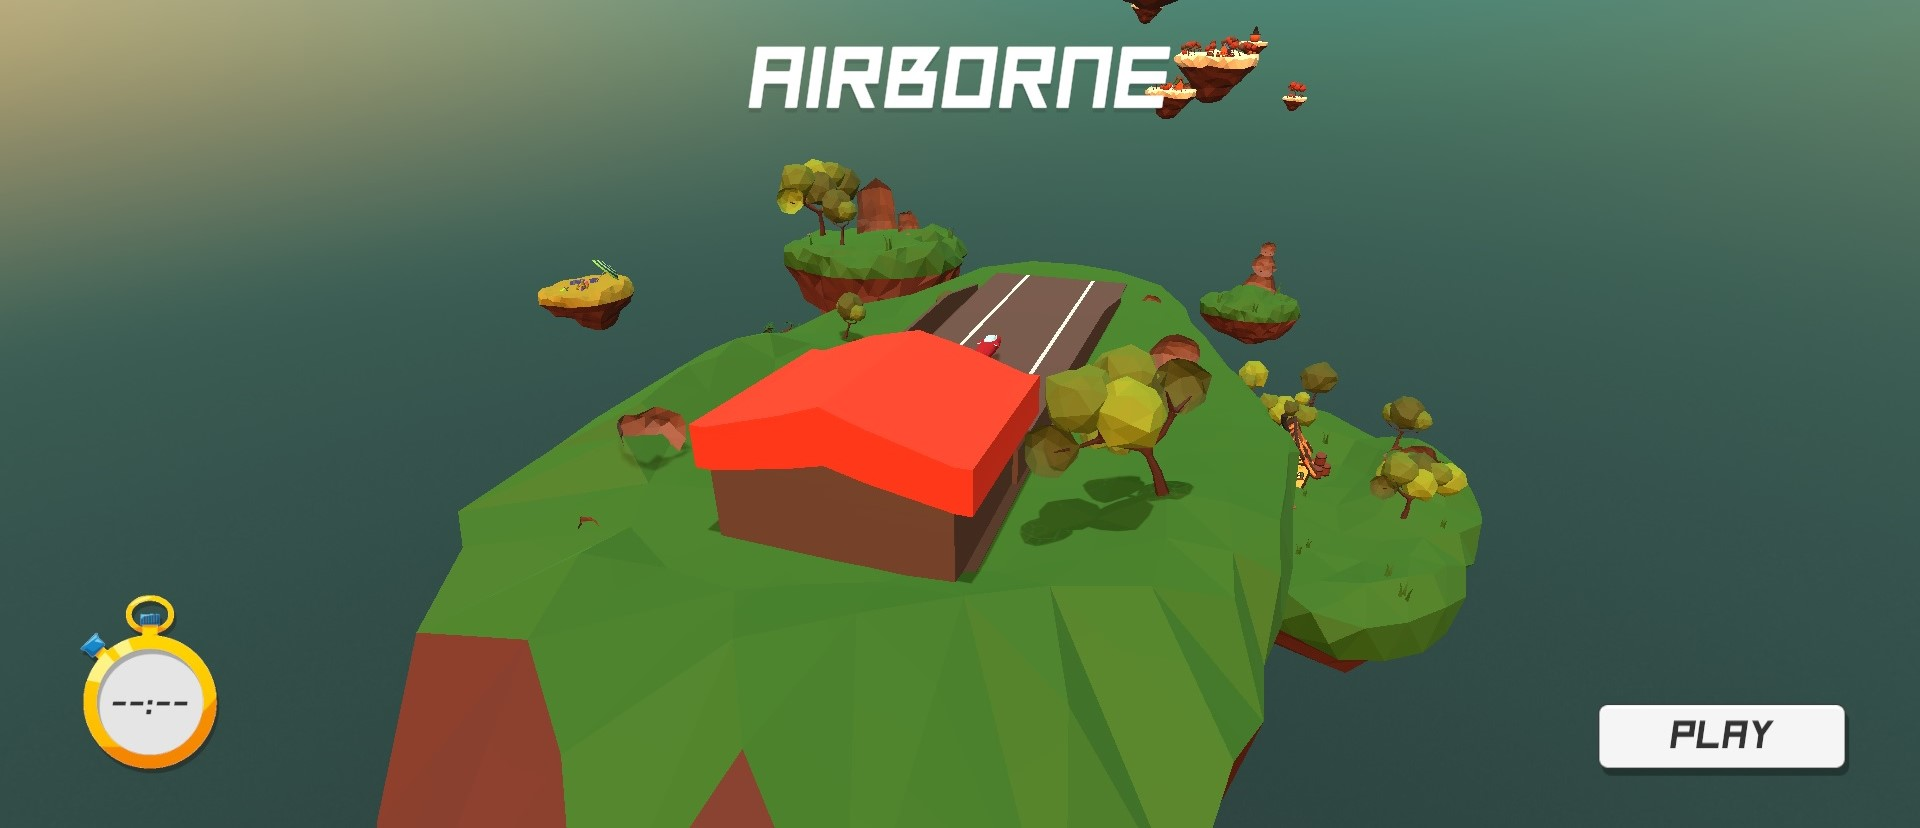
\includegraphics[width=\columnwidth]{mainmenu.jpg}
\end{center}

\begin{center}
     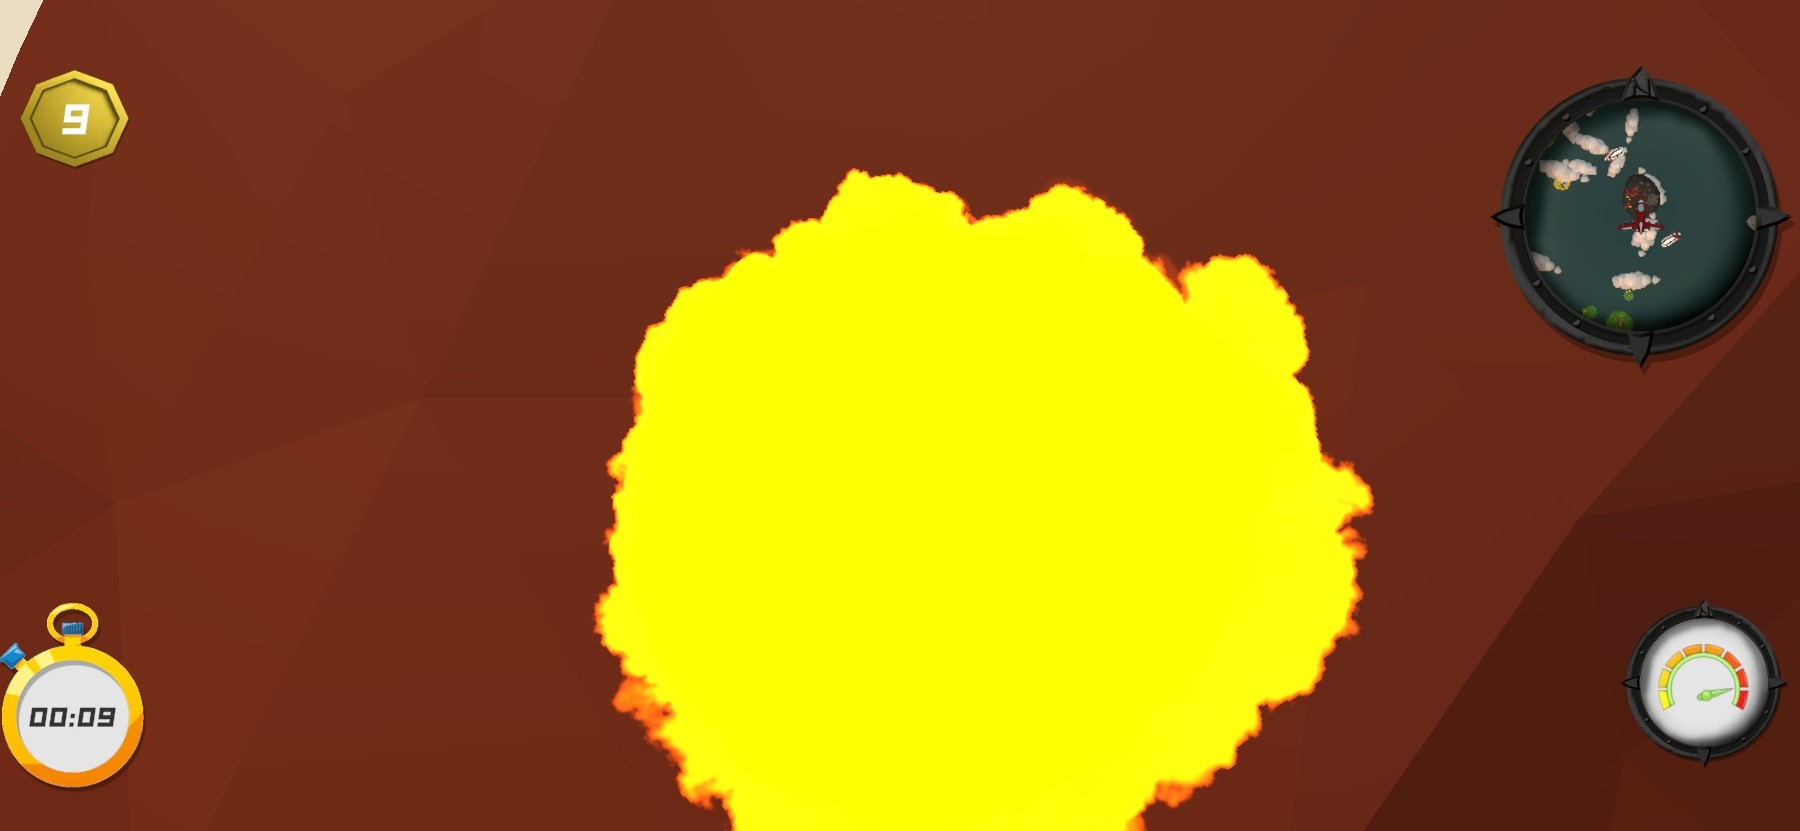
\includegraphics[width=\columnwidth]{eksplozija.jpg}
\end{center}

\section{Tehnični vidiki igre}

\subsection{Unity Scene}
V Unityju je igra razdeljena v 2 glavni sceni - MainMenu (glavni meni, kamor se igralec postavi na začetku in koncu) in GameScene (samo območje igranja).

\subsection{Let rakete}
Raketa se giblje po xyz oseh. Glede na pospešek in smer nanjo dodamo sile (AddTorque, AddForce). Koti se računajo z kvaternioni.

\subsection{Pozicija kamere}
Kamera se glede na pritisnjeno tipko in gibanje rakete pozicionira in rotira na tarčo (raketo). Spreminjamo vidljivost tarče. Koti se računajo z kvaternioni.

\subsection{Trki}
Za zaznavanje trkov uporabljamo dodelan Unityjev Collision detection z Colliderji in Particle System za proženje efektov oz. akcij ob trkih.

\subsection{Naključno generiranje}
V igri se na naključnih mestih z naključnim skaliranjem in smerjo premikanja generirajo samo oblaki. Žetoni in kantice goriva niso naključne z razlogom, da je igra pravična v smislu, da vedno tekmuješ le po času.

\subsection{Animacije}
Dodali smo animacijo ogenjčka rakete (ki se povečuje skupaj s pospeškom) in animacijo ognjene eksplozije ob trku oz zmanjkanju goriva. Prav tako se animirano premikajo oblaki in zeppelin.

\section{Zaključki in možne nadgradnje}
V tem seminarju smo po našem mnenju dosegli, kar smo si zastavili. Vključili smo več efektov in animacij, bolj gladek gameplay, predmeti so bolj zanimivi in posledično je uporabniška izkušnja toliko boljša. Največje težave so se pojavljale pri inkorporiranju določenih Blender elementov, prilagajanju fizike gibanja, usklajevanje projekta na različnih računalnikh z različnimi Unity verzijami in nasploh odpravljanje napak v kodi. Z našim izdelkom smo zadovoljni.

\section{Povezava do prenosa igre -WebBuild, WindowsBuild in gameplay}
{\url{https://we.tl/t-WmKnDPxFeZ}}
OPOMBA: Povezava preteče v roku 7ih dni.


\small
\bibliographystyle{plain}

\end{document}
